\documentclass[a4paper, 12pt]{article}
\usepackage[T1]{fontenc}
\usepackage[utf8]{inputenc}
\usepackage{booktabs}
\usepackage{titling}
\usepackage{titlesec}
\usepackage{amssymb}
\usepackage{pifont}
\usepackage{graphicx}
\graphicspath{ {../../} }

\usepackage{hyperref}
\hypersetup{
    colorlinks=true,
    linkcolor=black,
    urlcolor=cyan,
}
\urlstyle{same}

\renewcommand{\contentsname}{Obsah}
\renewcommand{\thesection}{\Roman{section}}
\renewcommand{\thesubsection}{\roman{subsection}}
\renewcommand{\thesubsubsection}{\roman{subsection}.\roman{subsubsection}}

\titleformat{\section}
{\Large\bfseries}
{\thesection}
{0.5em}
{}


\titleformat{\subsection}
{\large\bfseries}
{\thesubsection.}
{0.5em}
{}

\titleformat{\subsubsection}
{\large\bfseries}
{\thesubsubsection}
{0.5em}
{}

\title{
        \vspace{1in}
        \rule{\linewidth}{0.5pt}
		\usefont{OT1}{bch}{b}{n}
        \huge Programátorská dokumentace \\GrainSim\\
        \vspace{-10pt}
        \rule{\linewidth}{1pt}
}
\author{
		\normalfont\normalsize
        Marek Bečvář\\[-3pt]\normalsize
        31.7.2021
}
\date{}


\begin{document}
\maketitle 
\newpage

\tableofcontents
\newpage

\section{Rozbor specifikací} 
\subsection{Popis}
\paragraph{} 
Projekt GrainSim měl za cíl vytvořit v jazyce C\# a frameworku Monogame 2D
herní prostředí, ve kterém si uživatel bude moci tvořit experimenty s látkami, 
jejichž vlastnosti budou založené na těch reálných. V prostředí pak mohou
látky jak navzájem, tak v reakci na prostředí reagovat (výbušniny, hořlaviny,
přeměny skupenství, atd.).

\subsection{Funkční požadavky}
\emph{(z finální verze specifikace zápočtového projektu)}\\
\\
Na základě uživatelem vložených prvků aplikace:
\vspace{-5px}
\begin{itemize}
    \item vykresluje aktuální mapu prostředí 
    \item očekává další vstup od uživatele (výběr jiného prvku, změna
        vykreslovací mapy, aj.)
    \item v každém kroku simulace:
        \begin{itemize}
            \item přesouvá podle daných pravidel prvky po prostředí
            \item přepočítává teplotní mapu prostředí
            \item kontroluje prvky na možné reakce (na základě okolních prvků a
            teplot)
        \end{itemize}
\end{itemize}

\newpage
\section{Architektura/Design}
\small{\emph{Architektura programu byla před zahájením projektu načtrtnuta do
        UML grafu (které se v průběhu práce na projektu někdy rozrostlo, ale 
        velké změny nikdy nenastaly). To co si určitě z tohoto kurzu odnesu dál 
        je síla takového náčrtu, kdy člověk dokáže vyřešit problémy v architektuře 
daleko dříve, než se k nim vlastně dostane.}}

\begin{center}
    \hspace*{-80px}
    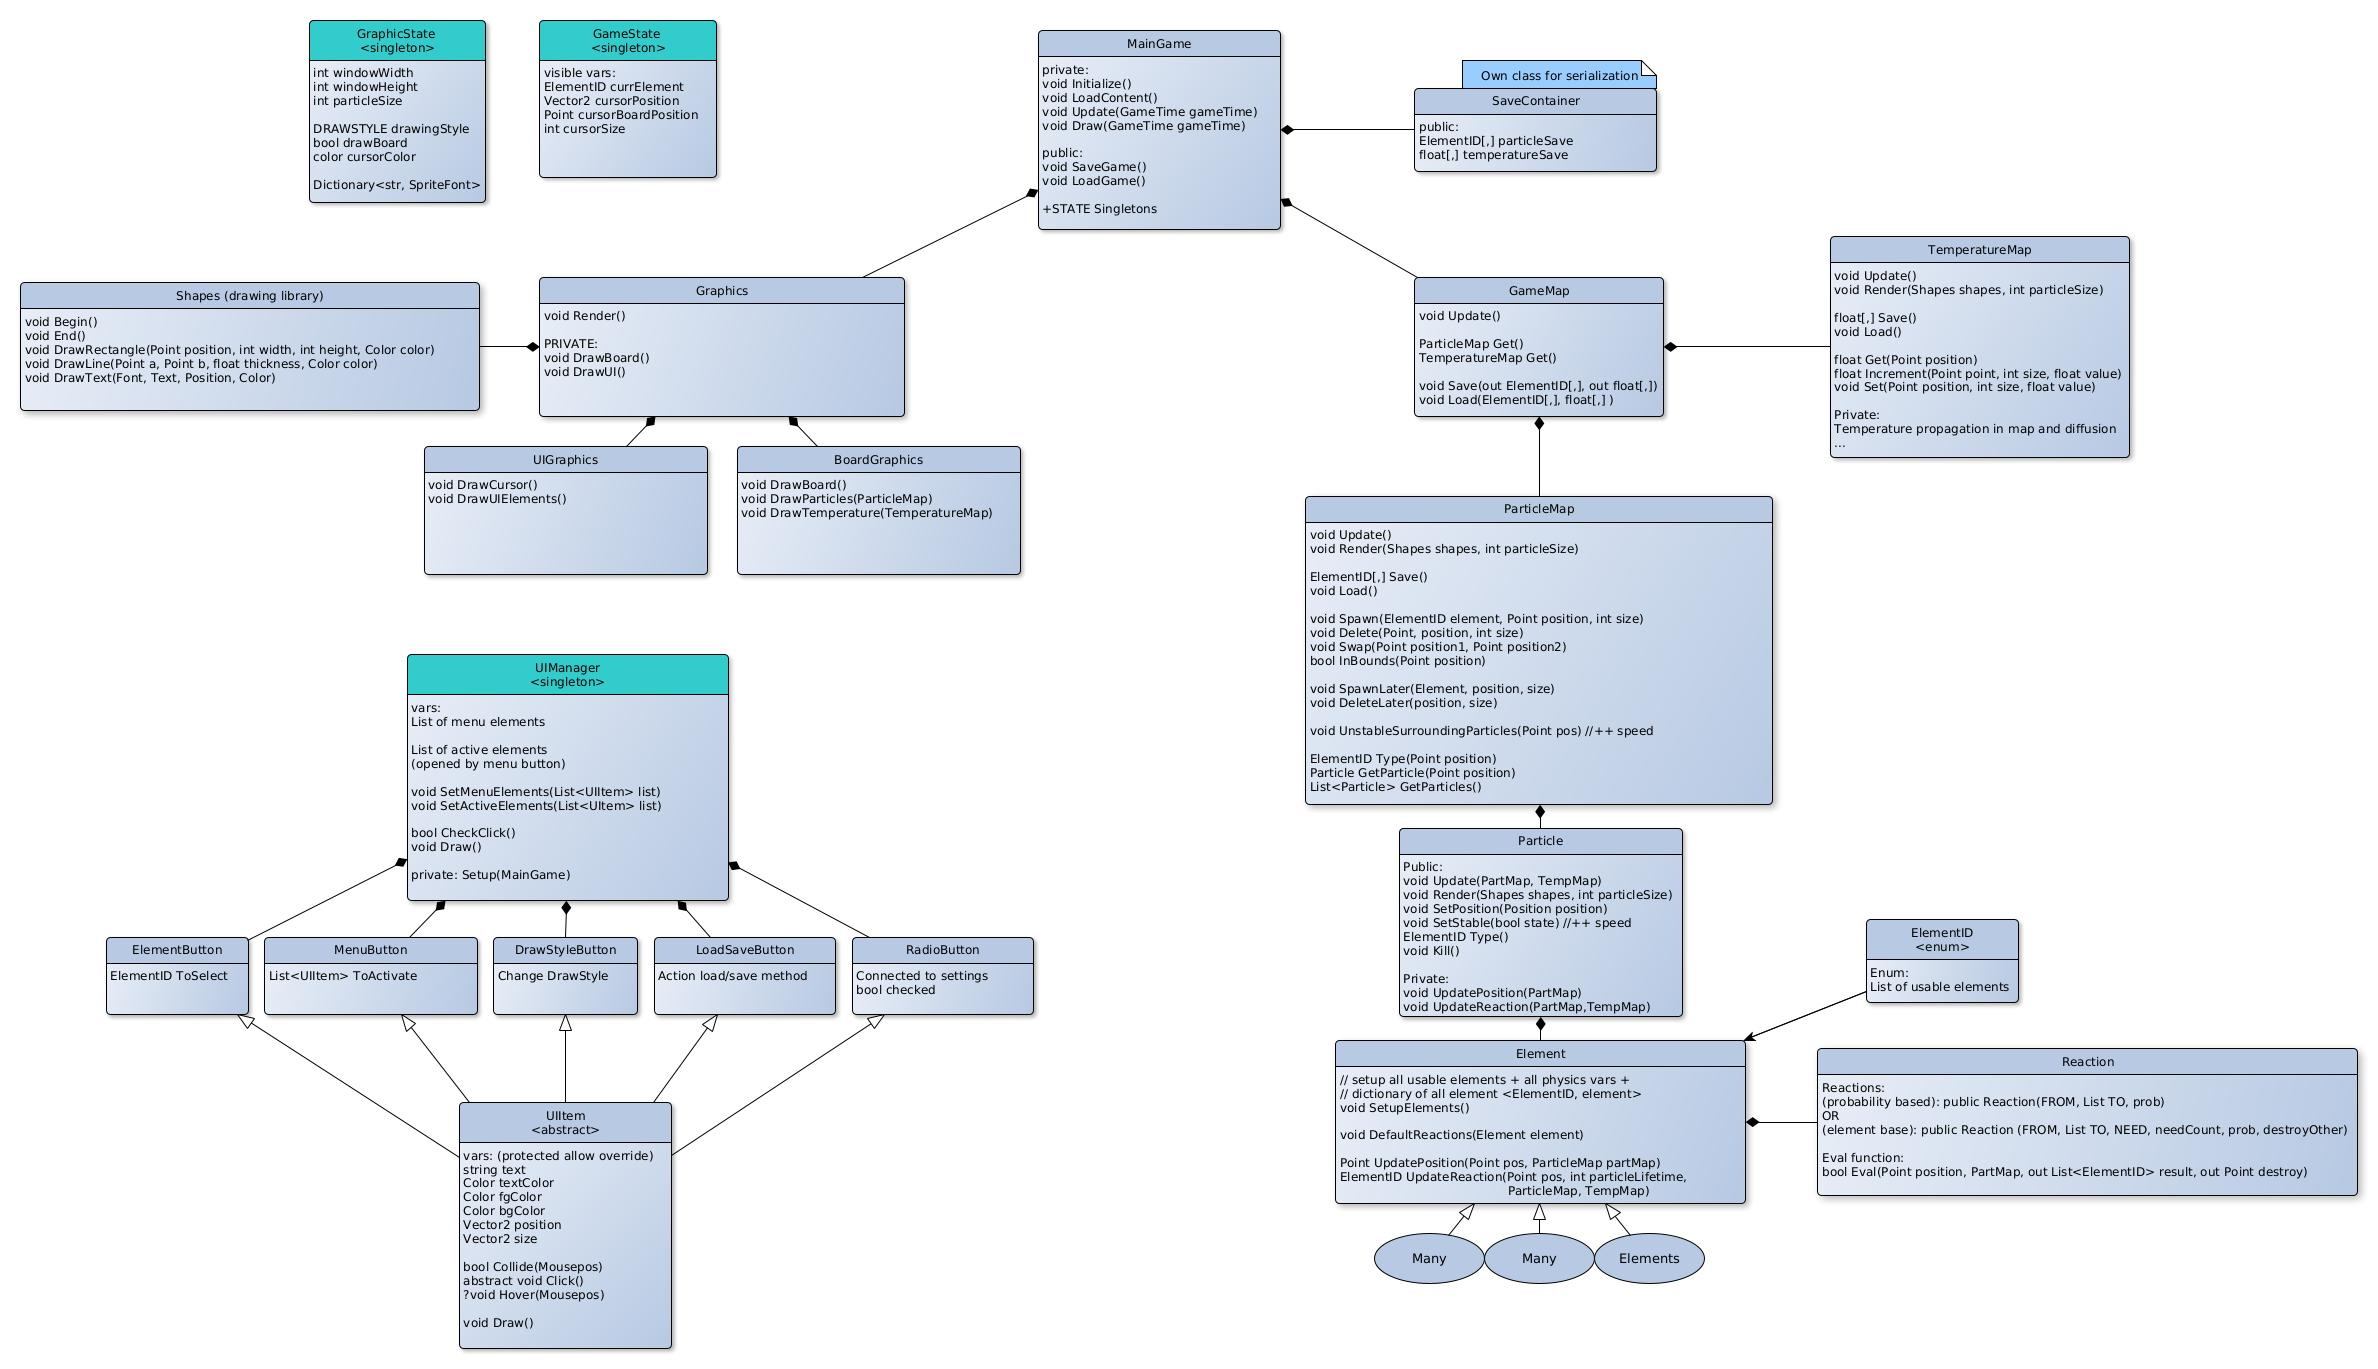
\includegraphics[width=1.4\linewidth]{GrainSim.jpg}
\end{center}

\paragraph{Rozdělení}
Celý program se dělí na více částí. Centrální je ale třída \texttt{MainGame}.
Zde se nachází veškerá logika spojená s Monogame. Zároveň se ale z tohoto
místa posílají výzvy k aktualizacím a vykreslení prostředí a výsledky
uživatelských vstupů. 

\newpage
\subsection{High-level}
\paragraph{Prvky/Teploty}
Centrální třídou kde se inicializují všechny potřebné části je
\texttt{MainGame}. Práce s prvky a teplotami probíhá ve speciálních mapách,
tudíž na \texttt{MainGame} navazuje třída \texttt{GameMap}, která v sobě drží
odkazy na mapu částic (\texttt{ParticleMap}) a mapu teplot
(\texttt{TemperatureMap}). Mapa částic pak v sobě má seznamy všech aktuálně
simulovaných prvků. Každý takto simulovaný prvek je popsán pomocí vlastní
instance třídy \texttt{Particle}. Jednou z hlavních vlastností této instance je
typ elementu, který představuje. Všechny možnné typy částic jsou pak popsané v
enum \texttt{ElementID} v tříde \texttt{Element}. Tato třída se stará o
veškerou inicializaci jednotlivých prvků, logiku jejich pohybu po mapě a řeší
jejich možné reakce, které jsou popsané vlastní třídou \texttt{Reaction}.
Jednotlivé prvky jsou pak vytvářené jako třídy odvozené od třídy
\texttt{Element} (každý prvek vlastní soubor) a jsou jim ručně nastaveny jejich
vlastnosti.

\paragraph{Vykreslování}
Zpět v třídě \texttt{MainGame} se nachází odkaz na třídu \texttt{Graphics}, což
je centrální třída pro vykreslování všeho. Pod ní se nachází třída
\texttt{Shapes}, což je vlastní třída pro vykreslování tvarů a textu na
obrazovku. Dále má tato třída odkaz na třídy \texttt{UIGraphics} a
\texttt{BoardGraphics}. \texttt{UIGraphics} může inicializovat vykreslování
jednotlivých UI prvků (menu, infotext) a zároveň řeší vykreslování kurzoru.
\texttt{BoardGraphics} může vykreslovat čtverečkovanou sít a mapy částic a
teplot.

\paragraph{UIManager}
O logiku a vlastní vykreslování UI elementů v menu sekci se stará vlastní
singleton \texttt{UIManager}, který pod sebou má řadu různých typů tlačítek,
odvozené od abstraktní třídy \texttt{UIItem}.

\paragraph{State singletons}
Pro určité speciální hodnoty programu jsem vytvořil dva \\singletony (\emph{zejména
protože se jedná o velmi specifické parametry potřebné skoro všude a jejich
předávání by akorát přineslo větší zmatek do funkcí}). Jedná se o
\texttt{GraphicState} (hodnoty velikosti herního okna, zvolená
velikost částic, zvolený typ vykreslování, toggle vykreslování čtverečkované
sítě, barvu kurzoru a list načtených fontů) a \texttt{GameState} (právě zvolený
element, pozice myši na obrazovce, přepočet pozice myši do čtverečkované plochy
a aktuální velikost kurzoru).

\newpage
\subsubsection{Mapování na funkční požadavky}
\begin{itemize}
    \item vykresluje aktuální mapu prostředí \(\rightarrow\) \texttt{Graphics} a připojené
        třídy
    \item očekává další vstup od uživatele (výběr jiného prvku, změna
        vykreslovací mapy, aj.) \(\rightarrow\) \texttt{MainGame} s \texttt{UIManager}
    \item v každém kroku simulace: \(\rightarrow\) skrz třídu \texttt{GameMap}
        \begin{itemize}
            \item přesouvá podle daných pravidel prvky po prostředí \(\rightarrow\)
                \texttt{ParticleMap} a vlastní třída \texttt{Element}
            \item přepočítává teplotní mapu prostředí \(\rightarrow\) celé v třídě
                \texttt{TemperatureMap}
            \item kontroluje prvky na možné reakce (na základě okolních prvků a
                teplot) \(\rightarrow\) třídy \texttt{Element} a \texttt{}
        \end{itemize}
\end{itemize}

\section{Rozdělení do funkcí a procedur}
\paragraph{Update}
Všechna volání procedur vychází opět z hlavní třídy \texttt{MainGame}.
Zde se nachází dvě procedure základem v Monogame frameworku \texttt{Update} a
\texttt{Draw}. V \texttt{Update} se řeší uživatelské inputy (v
\texttt{UIManager.CheckClick}) a zároveň se odtud volají update procedury ve třídě
\texttt{GameMap}, které se dále propagují do updatů tříd jednotlivých map a v
mapě částic až do jednotlivých částic. V částicích se pak volají funkce třídy
\texttt{Element} s připojením daného typu částice, které řeší pohyb částice a
její možné reakce (\emph{tato volání jsou velmi drahá s narůstajícím množstvím
    částic, a proto se částice, která neprochází změnami polohy ani stavu, po 
    několika takových cyklech uspí a probouzí se, až když nastane nějaká aktivita v okolních částicích}).

\paragraph{Input handle}
Při hodnocení uživatelského vstupu se nejprve kontroluje, jestli nebylo
stisknuté nějaké tlačítko klávesnice poté jestli nebylo stisknuté tlačítko v
menu části - konrola v \texttt{UIManager.CheckClick} a pokud ne, tak kontrola,
jestli neprobíhá stisk levého nebo pravého tlačítka na simulačním prostředí.

Pokud ano, pak se na základě právě zvoleného prvku rozhoduje předávání události
do speciálních metod tříd \texttt{TemperatureMap} nebo \texttt{ParticleMap}.
Ty si řeší uživatelský vstup samostatně na základě pozice kurzor v mapě a
velikosti kurzoru.

\paragraph{Draw}
Na druhou stranu \texttt{MainGame} vysílá se zvé \texttt{Draw} procedury volání
na \texttt{Graphics.Render}, kde se vyhodnocuje, jaké vše vykreslovací metody v
\texttt{UIGraphics} a \texttt{BoardGraphics} zavolat. \texttt{UIGraphics} toto
volání poté přesouvá na singleton \texttt{UIManager}, který drží všechna
tlačítka potřebná k vykreslení a volá jejich vlastní \texttt{Draw} metody
odvozené od abstraktní třídy \texttt{UIItem}.
\texttt{BoardGraphics} vykreslování částic i teplot také předává do
jednotlivých map, které mají vlastní logiku vykreslování ve svých
\texttt{Render} funkcích.

\newpage
\section{Implementované datové struktury}
\paragraph{}
Program nemá žádné speciální datové struktury. Užitečnými byly struktury
\textbf{dictionary}, \textbf{list} a \textbf{víceúrovňové pole}.

\paragraph{Víceúrovňové pole}
Víceúrovňové pole se využívá pro indexování buněk mapy částis a pro udržení a
práci s hodnotami teplot v mapě teplot.

\paragraph{List}
Datová struktura list je použita třeba pro obecné reakce jednotlivých elementů.
Při inicializaci těchto elementů tak stačí do listu pouze naskládat kolik
různých reakcí chceme a procedura třídy \textbf{Element} pak při kontrole
reakcí všechny tyto načtené kontroluje.

Dále je list využíván v menu stavech. \texttt{UIManager} udržuje listy tzv.
\emph{menu elementů} (= velká tlačítka, kategorie) a \emph{aktivních elementů}
(= menší tlačítka, př. samotné elementy, možnosti nastavení). Dále pak existuje
typ tlačítka \texttt{MenuButton}, který v sobě obsahuje list tlačítek a
kategorii, do které mají být načtena. Takto je možno s předáváním dvou listů
vytvářet v podstatě libovolně hluboké menu (\emph{jen možná inicializace těchto
tlačítek může být trochu nepřehledná - \texttt{MainGame.Setup}}).

\paragraph{Dictionary}
Dictionary je v tomto programu využito také na více místech. \\Důležitá je
globální proměná \texttt{Element.elements}, která s klíčem z enum
\texttt{ElementID} odkazuje na jednotlivé třídy vlastních prvků (\emph{tak je možné
se dostat k vlastnostem jednotlivých elementů bez potřeby všude předávat velké
odkazy na celé třídy prvků}).

Dále je dictionary využita v mapě částic pro udržení a spravování aktivních
částic. Zde je klíčem index pozice v mapě, na kterém se prvek nachází (\emph{při
pohybu se částice vyměňují na pozicích, index pozice mapy je po celou dobu
stejný}). Původní implementace využívala list, ale udělal jsem přechod k 
dictionary z důvodu rychlostní převahy. V simulaci se obvykle nachází okolo
5000 částic a při potřebe odebrat z takového listu třeba 100 položek (při
dostatečně velkém kurzoru možné) na úplně neznámých indexech, je rychlostně
naprosto nezvladatelné. Proto bylo zvolené dictionary. Zjistit klíče, se kterým
chci pracovat je jednoduché (z pozic v mapě - díky pozici kurzoru znám).
Indexování pomocí klíče by poté bylo to nejrychlejší co může program nabídnout.
Zároveň, dictionary je celé vytvořené a zaplněné při inicializaci, tudíž už
nedochází k žádnému opakovanému vytváření. Stačí zvolit množstvím částic, které
je zvladatelné a simulace nebude mít s daným počtem částic žádné problémy.

Posledním místem, kde je tato struktura využita je v \texttt{GraphicState} jako
kontejner na použitelné fonty textu inicializované v \texttt{MainGame}. Klíčem
k nim jsou v kódu zvolené proměnné, popisující využití těchto fontů.


\newpage
\section{Závěr}
\paragraph{}
Projekt byl vytvoření jako záverečná semestrální práce pro předmět
\\\emph{Programování 2} - Letní semestr 2021 - UK Matfyz.
\end{document}

